\documentclass[12pt,a4paper]{article}
\usepackage[utf8]{inputenc}
\usepackage{amsmath}
\usepackage{amsfonts}
\usepackage{amssymb}
\usepackage{minted}
\usepackage{graphicx}
\usepackage[linesnumbered,ruled,vlined]{algorithm2e}
\usepackage[margin = 2.00cm]{geometry}
\usepackage{tikz}
\author{GHAOUI Anis}
\title{Compte rendu TP A3}


\SetKwInput{KwInput}{Input}                % Set the Input
\SetKwInput{KwOutput}{Output}              % set the Output


%
\newcommand{\inputvhdl}[1]{\inputminted[linenos,tabsize=2]{vhdl}{./src/#1.vhd}}

\begin{document}
%page de garde Quentin
\section{Introduction}
La complexité de la conception des systèmes embarqués modernes étant devenue trop élevée, il est indispensable de recourir à des outils afin d'automatiser ce processus fastidieux. Dans le cours A3, on voit que les étapes de cette conception consistent en la préparation d'un système ayant un CPU virtuel dit \textit{SoftCore}, une ou plusieurs mémoire pour accompagner ce CPU et une brique FPGA qui agit comme un accélérateur matériel. Durant les séances de TP, on procède à la conception de plusieurs variante cette brique afin d'effectuer le calcul d'une racine carrée entière sur FPGA décrite en VHDL. Puis, on instancie un système embarqué grâce à l'outil Qsys d'Intel/Alter pour avoir un CPU et les périphériques requis. Enfin, on intégrera la brique conçue dans ce système afin de mesurer ses performances globales.

\section{Conception d'opérateur racine carrée}
On commence par une analyse de l'algorithme afin de comprendre sa complexité et l'utilité d'accélérer un tel calcul matériellement.

\begin{algorithm}[H]
	\KwInput{(X,n) : X  entier codé sur $2\times n$ bits}
	\KwOutput{Z : Z entier codé sur n bits}
	Charger X
	
	$V = 2^{2n-2}$
	
	$Z=0$
	
	\For{i = n-1 à 0}{
		$Z =Z+V$
		
		\If{$X-Z\ge 0$}{
			$X=X-Z$
			
			$Z= Z+V$
		}
		\Else 
		{
			$Z=Z-V$
		}
		$Z=Z/2$
		
		$V=V/4$		
	}
	retourner Z
\end{algorithm}
%Q, ajoute des trucs

\subsection{Implémentation combinatoire}
Dans un premier temps, on pense à simplement traduire \textbf{tout} l'algorithme en vhdl dans un seul \textit{process} afin d'avoir une séquence d'éléments combinatoires propageant le résultat pour chaque valeur de i. Ceci sera synthétisé comme un circuit volumineux très lent.
\paragraph{Résultats}
%diag temporel et commentaire
\paragraph{Code}
\inputvhdl{SQRT_one_process}

\subsection{Implémentation multi-cycles}
\subsubsection{4 cycles}
On choisit alors d'implémenter une machine synchrone où on décrit le module de racine carrée par une machine d'états finis. il y aura un cycle où on itère $n$ fois . Le diagramme ci-dessous représente cette automate :
\begin{figure}[H]
\centering
\tikzstyle{nodus}=[circle,draw=black,minimum size=1.75 cm]
\def\dis{2}
\begin{tikzpicture}
\node [nodus] (wait)	[label={[label distance=0.5cm]90:!start}]  at (0,0) {wait};
\node [nodus] (init) 	[right of = wait,right = \dis cm] {init};
\node [nodus] (iter) 	[label={[label distance=0.5cm]-60:i!=n}]  [below of = init,below=\dis cm] {iter};
\node [nodus] (end) 	[below of = wait,below= \dis cm] {end};
\node [nodus] (default) [left of = wait,left = \dis cm] {default};

\draw [->] (wait) edge node [midway,above]{start}  (init);
\draw [->] (init)   edge (iter);
\draw [->] (iter)  edge node [midway,above]{i==n}  (end);
\draw [->] (end) edge (wait);
\draw [->] (default) edge (wait);

\draw [->](wait)  to[distance = 1 cm ,out=45,in=135] (wait);

\draw [->](iter)  to[distance = 1 cm ,out=-45,in=-90] (iter);

\end{tikzpicture}
\end{figure}
%explication des états

\subsubsection{9 cycles}
Cette implémentation décompose relativement bien les états de l'automate. Mais, on pense pouvoir obtenir un gain de performances en ayant un cycle par opération à effectuer. L'idée est que vu que l'état sera combinatoirement simple, il sera plus rapide  à exécuter et donc la fréquence augmente. Par contre, on pense aussi que ceci consommera plus de ressources du FPGA.
\begin{figure}[H]
	\centering
	\tikzstyle{nodus}=[circle,draw=black,minimum size=1.5 cm,text width=1.5cm,align=center]
\def\dis{1.5}
\begin{tikzpicture}
\node [nodus] (wait)	[label={[label distance=0.5cm]90:!start}]  at (0,0) {wait};
\node [nodus] (init) 	[right of = wait,right = \dis cm] {init};
\node [nodus] (end) 	[below of = init,below= \dis cm] {end};
\node [nodus] (default) [below of = wait,below= \dis cm] {default};
\node [nodus] (iter1) [right of = init, right= \dis cm] {Rz+Rv};
\node [nodus] (iter2) [right of = iter1, right= \dis cm] {compare = Rx-Rz};

\node [nodus] (iter3_bis) [below of = iter2,below= \dis cm] {Rz-Rv};

\node [nodus] (iter3) [right of = iter2, right= \dis cm] {Rx-Rz};
\node [nodus] (iter4) [below of = iter3, below= \dis cm] {Rz+Rv};
\node [nodus] (iter5) [left of = iter3_bis, left= \dis cm] {Rz/=2 Rv/=2};


\draw [->] (wait) edge node [midway,above]{start}  (init);
\draw [->] (init)   edge (iter1);
\draw [->] (iter1) edge (iter2);
\draw [->] (iter2) edge node [rotate=60,midway,right]{$compare >= 0$}(iter3);
\draw [->] (iter3) edge  (iter4);
\draw [->] (iter4) to [in=-45,out=-135] (iter5);
%%%%%
\draw [->] (iter2) edge node [midway, right]{$compare < 0$}(iter3_bis);
\draw [->] (iter3_bis) edge (iter5);
%%%%%
\draw [->] (iter5) edge node [midway,below] {$i==1$}(end);
\draw [->] (iter5) edge node [midway,right] {$i > 1$} (iter1);

%\draw [->] (iter)  edge node [midway,above]{i==n}  (end);
\draw [->] (end) edge (wait);
\draw [->] (default) edge (wait);

\draw [->](wait)  to[distance = 1 cm ,out=45,in=135] (wait);


\end{tikzpicture}
\end{figure}
\subsubsection{Variante avare} %Quentin

%

\subsection{Implémentation avec opérateur unique}
On propose alors une implémentation avec un seul addition/soustracteur proposé dans l'énoncé. Ceci a pour but de diminuer le nombre d'éléments logiques utilisés. Il existe plusieurs implémentations de cet opérateur qui ont toutes comme contraintes de n'instancier qu'un seul opérateur qui est fourni par l'énoncé.

\subsubsection{Opérandes préemptées}
Dans cette variante, on positionne les variables à l'entrée de l'opérateur à un cycle avant leur utilisation. Ceci va contraindre la synthèse à avoir une période d'horloge plus grande que la durée de l'opération combinatoire d'addition/soustraction.

\subsubsection{Ségrégation des machines} % Quentin

\subsection{Implémentation Pipeline} % Quentin

\section{Comparaison et résultat}
On remarque qu'il existe plusieurs compromis en termes de fréquences, surface FPGA. On peut par ailleurs comparer les différentes implémentations entre elles. On obtient ainsi les résultats suivants.
\begin{figure}[H]
	\centering
	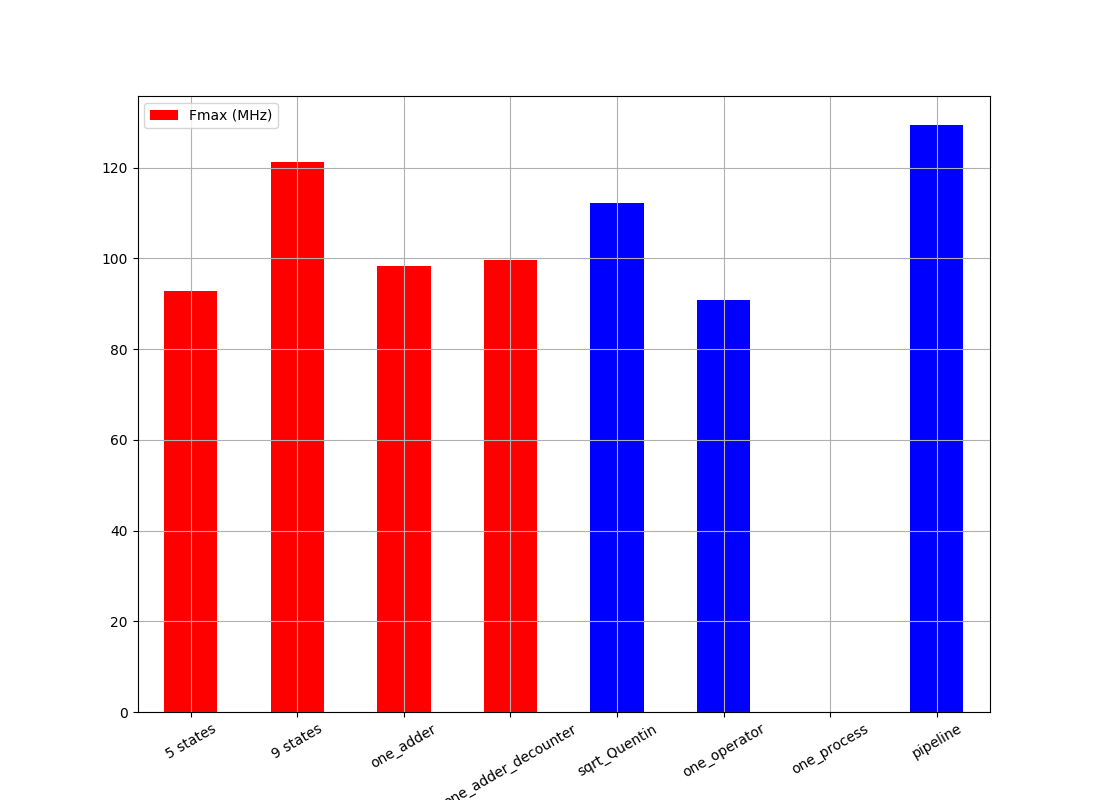
\includegraphics[width=0.7\linewidth]{mesures_freq/0}
	\caption{Mesures fréquentielles des différentes implémentations }
	\label{fig:0}
\end{figure}
On ne peut pas mesurer la fréquence de fonctionnement d'une circuit combinatoire sans imposer de registres à l'entrée et la sortie du circuit. On remarque que, comme attendu, on a un pipeline cadencé à une vitesse plus importante que les autres circuits. On remarque aussi que les circuits multi-cycles sont plus rapides que les circuits mono-opérateur. Ce qui est logique car elles prennent plus de place afin d'assurer une telle cadence.
\begin{figure}[H]
	\centering
	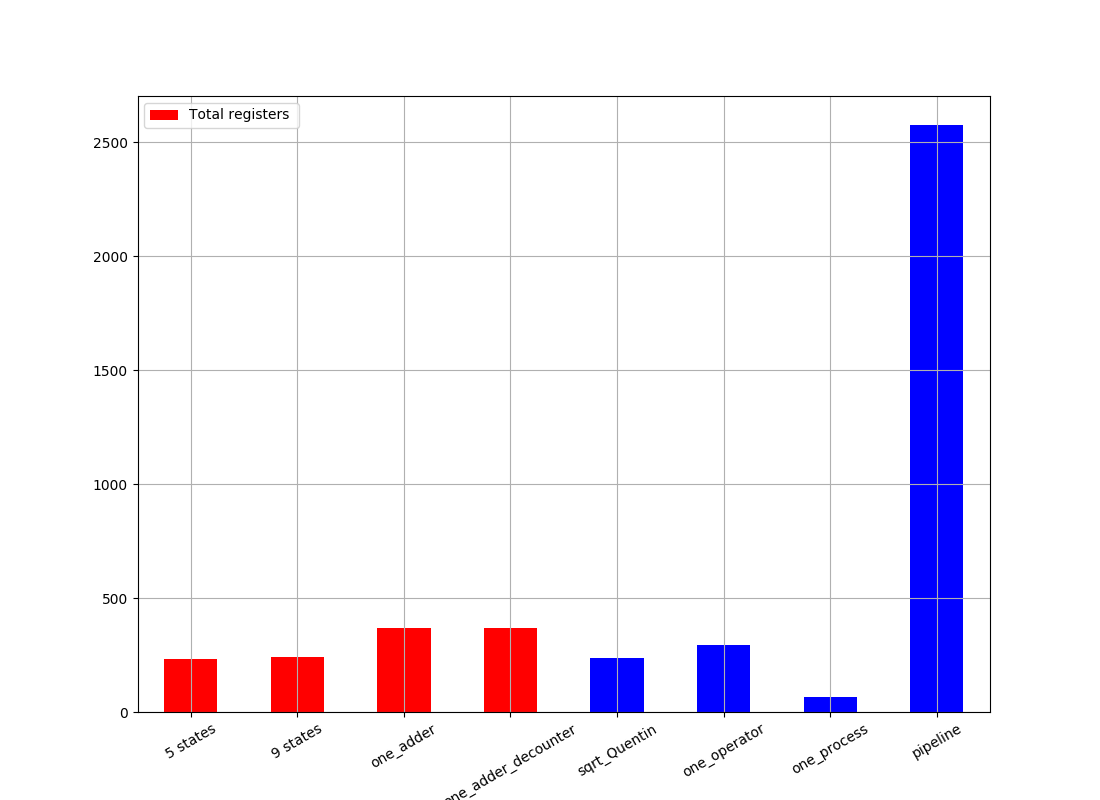
\includegraphics[width=0.7\linewidth]{mesures_freq/4}
	\caption{Usage de la surface FPGA par circuit implémenté}
	\label{fig:1}
\end{figure}
En terme de surface et éléments logiques occupés, la figure \ref{fig:1} montre que le pipeline occupé effectivement n fois plus de ressources car il y a bien n étages du même circuit. Aussi, on confirme bien les résultats trouvés en fréquentiel en observant que les mono-opérateurs sont plus économique en terme de surface FPGA.

\section{Conception du système embarqué} % 23-Jan
Le système embarqué sera implémenté sur une carte Intel/Altera Cyclone II De1. Au cœur de ce système : un softcore le NIOS2 entouré de contrôleurs mémoires On-chip, SDRAM, SSRAM, module racine carrée VHDL et bien-sûr le périphérique JTAG permettant de programmer et déboguer le NIOS. Par ailleurs, on utilisera des IP préconçues qui vont accélérer le développement du système. 


\subsection{Implémentation et programmation du Nios}
L'IP du softcore est fourni par Intel/Altera en plusieurs versions chacune offrant différentes cadences fréquentielles, caches instructions/données, opérateurs et pipeline. On ne détaillera pas ces différences ici car elles ont été vu en cours et peuvent être retrouvées dans la documentation d'Intel. On implémente donc les différentes versions telles que :
\begin{itemize}
\item Nios e : cache instructions 512 o
\item Nios s : cache instructions 512 o et données 512 o
\item Nios s : cache instructions 2 ko et données 2 ko
\item Nios f : cache instructions 512 o et données 512 o
\item Nios f : cache instructions 2 ko et données 2 ko
\end{itemize}
\subsection{Usage des différentes mémoires}
Grâce aux outils de développement proposés par Intel/Altera, on peut semi/automatiquement instancier de systèmes embarqués avec la possibilité de paramétrer l'emplacement mémoire du programme qui sera exécuté sur CPU. On peut alors écrire un programme qui calcule la racine carrée entière d'un nombre de manière logicielle, i.e. utiliser les opérateurs du NIOS. Ensuite, placer les données et le code dans soit la mémoire On-chip, SSRAM ou SDRAM. Ceci permet d'établir un comparatif entre ces différentes mémoires en termes de conception et timings pour plusieurs version du NIOS vues en cours. 

%Quentin ajoute ce que tu penses pértinant

\subsection{Comparaison des différentes implémentations}
On exécute le même programme C sur les différentes version du Nios. On mesure à chaque fois le temps d'exécution de ce code pour une mémoire et un version Nios.

\subsubsection{Mesure de temps}
Il existe plusieurs manières de mesurer le temps d'exécution sur Nios. Dans notre cas, on peut soit utiliser la bibliothèque fournie par le constructeur afin d'exploiter le registre compteur du Nios. Ou bien, implémenter nous-même ces fonctions de mesures afin d'avoir un plus grand contrôle sur la mesure de temps. Sans détailler, on opte pour implémenter ces fonctions et on les compare avec la version proposée par Altera :
$$
\begin{array}{cc}
	Impl\acute{e}mentation & \textit{temps de mesure à  vide ms} \\ 
	Altera & 108 \\ 
	Personnalis\acute{e}e & 56 
\end{array} 
$$

On garde alors nos propres fonctions de mesures. On procède à une mesure fine du temps d'exécution. I.e. on  mesure le temps de lecture depuis un tableau, d'exécution de la fonction racine carrée et de l'écriture dans un tableau qui contient 1000 éléments. On obtient alors le tableau suivant :
\begin{table}[H]
	\centering
	\begin{tabular}{|c|c|c|c|c|}
		\hline
		Lecture (ms) & exécution (ms) & écriture (ms) & mémoire &  Nios  \\ \hline
		   951006    &     152117     &    143773     &  SDRAM  & 2k\_f  \\ \hline
		   920547    &     113891     &    107808     &  SSRAM  & 2k\_f  \\ \hline
		   864807    &     56543      &     52084     & ONCHIP  & 2k\_f  \\
		   \hline		  \hline
		  4408206    &     167321     &    174576     &  SDRAM  & 2k\_s  \\ \hline
		  1780954    &     86035      &     86012     &  SSRAM  & 2k\_s  \\ \hline
		  1332246    &     71018      &     71008     & ONCHIP  & 2k\_s  \\ 

		  \hline		  \hline

		  1021266    &     198997     &    142142     &  SDRAM  & 512\_f \\ \hline
		   946526    &     124316     &    102657     &  SSRAM  & 512\_f \\ \hline
		   911848    &     73247      &     57028     & ONCHIP  & 512\_f \\ 

		   \hline		  \hline

		  4407738    &     167296     &    174586     &  SDRAM  & 512\_s \\ \hline
		  1780954    &     86035      &     86012     &  SSRAM  & 512\_s \\ \hline
		  1332246    &     71018      &     71008     & ONCHIP  & 512\_s \\ 
		  \hline		  \hline

		  13484546    &     709816     &    713872     &  SDRAM  &   e    \\ \hline
		  5308056    &     316000     &    319000     &  SSRAM  &   e    \\ \hline
		  3992076    &     245000     &    248000     & ONCHIP  &   e    \\ \hline
	\end{tabular} 
\caption{Temps de lecture, d'exécution et écriture des différentes}
\end{table}
On remarque que la version 2k\_f du Nios est la plus performante. Ceci est évident car c'est elle qui exploite le plus la surface du FPGA et possède des opérateurs en pipeline plus profonds. La mémoire Onchip est plus rapide que la SRAM et encore plus rapide que la DRAM du fait de la nature de conception des ces mémoires et la rapidité des accès. On remarque aussi qu'il y a des masquages des latences du chargement par la version 2k\_f.

En terme de surface FPGA, on peu voir sur le graphe suivant que la surface occupée est liée à la version du Nios. Plus la version est performante, plus elle occupera de la surface.
\begin{figure}[H]
	\centering
	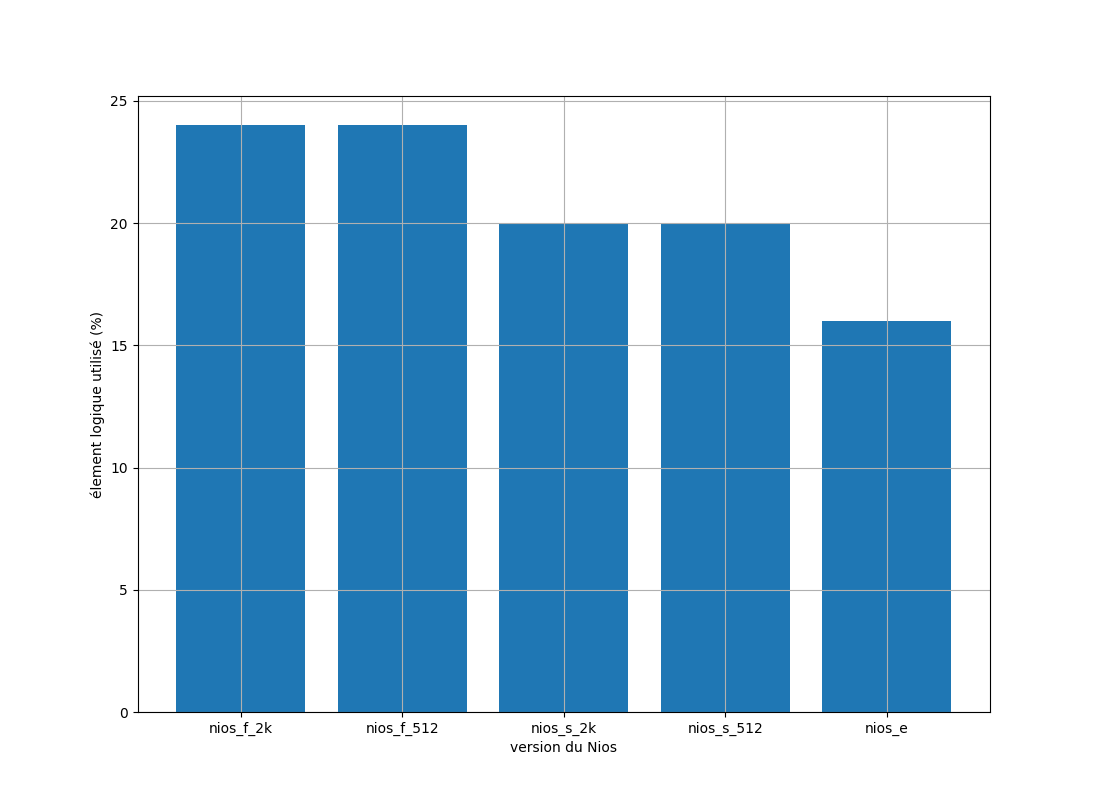
\includegraphics[width=0.75\linewidth]{figures/plot}
	\caption{Occupation des éléments logiques du FPGA}
\end{figure}
Les mêmes versions de nios occupent le même nombre d'éléments logiques mais un espace mémoire cache plsu grand.


\section{Intégration des instructions personnalisées}
\section{Intégration du coprocesseur}
\end{document}